\documentclass[10pt]{beamer}
% \setbeamercovered{transparent}
\beamerdefaultoverlayspecification{<+(1)-| alert@+(1)>}
\usetheme{Boadilla}
\usecolortheme{seahorse}
\usefonttheme{structurebold}
\usepackage{multicol}
\usepackage{graphicx}
\usepackage{tikz}
\usepackage{calc}
\usetikzlibrary{calc}
\usepackage{fp}
\usepackage{listings} % Pacote para destacar código fonte
\usepackage{amsmath} 
\usepackage{amssymb} 
\usepackage{helvet}
\usepackage{xcolor}
\usepackage{pgfplots}
\usepackage{array}
\usepackage{arydshln}
\usepackage{enumitem}
\pgfplotsset{compat=1.18}


\lstset{
  language=C++,
  basicstyle=\small\ttfamily,
  numbers=left, % Adiciona a numeração nas linhas
  numberstyle=\tiny, % Estilo da numeração (pequena)
  stepnumber=1, % Incremento da numeração
  numbersep=-30pt, % Espaçamento entre a numeração e o código (valor negativo)
}

\newcommand{\codecppNoTitle}[2][0.6]{
  \centering
  \begin{minipage}{#1\textwidth}
    %Referencia: https://ctan.dcc.uchile.cl/macros/latex/contrib/listings/listings.pdf
    \lstset{
      language=C++,
      numbers=left,
      numberstyle=\tiny,
      stepnumber=1,
      numbersep=5pt,
      showstringspaces = false,
      frame=shadowbox,
      commentstyle=\color{commentgreen},
      keywordstyle=\color{eminence},
      stringstyle=\color{red},
      backgroundcolor=\color{black!3},
      keywordstyle=\color{blue},
      rulesepcolor=\color{black!5},
      basicstyle=\small\ttfamily, % basic font setting
      emph={int,char,double,float,unsigned,void,bool},
      emphstyle={\color{blue}}
    }
    \lstinputlisting{#2}
  \end{minipage}}


% Definindo as cores para as palavras reservadas
\definecolor{keywordblue}{RGB}{0,0,255}
\definecolor{identifierblack}{RGB}{0,0,0}

\newcommand{\duascolunas}[2]{
  \begin{columns}
    \begin{column}{0.72\textwidth}
      #1
    \end{column}
    \begin{column}{0.28\textwidth}
		#2
	\end{column}
  \end{columns}
}

\title{Análise de Complexidade}
\author{Prof. Kennedy Reurison Lopes}
\date{\today}

% Início do documento
\begin{document}

\frame{\titlepage}

\begin{frame}
    \frametitle{Introdução}

    \begin{itemize}
        \item Bem-vindos à apresentação sobre a complexidade de realizar uma tarefa!
        \item Hoje discutiremos exemplos de tarefas que podem ser complexas, mesmo não necessariamente estejam diretamente relacionados a algoritmos.
        \item Depois iremos direto ao assunto: Como identificar a complexidade em algoritmos.
    \end{itemize}
\end{frame}

\begin{frame}
    \frametitle{Ordenar uma pilha de livros}
    \begin{itemize}
        \item Imagine uma pilha desorganizada de livros.
        \item A tarefa é organizá-los em ordem alfabética.
        \item A complexidade aumenta à medida que a pilha de livros fica maior.
    \end{itemize}
\end{frame}

\begin{frame}
    \begin{figure}[htb]
        \centering
        
\includegraphics[width=0.9\textwidth]{wally.jpg}
        \label{fig:wally2}
    \end{figure}
\end{frame}

\begin{frame}
    \frametitle{Encontrar um item específico}
    \begin{itemize}\large
        \item Suponha que você precise encontrar um objeto específico em uma sala cheia de itens.
        \item Quanto mais desorganizada a sala e mais objetos houver, mais complexa será a tarefa de localizar o item desejado.
    \end{itemize}
\end{frame}

\begin{frame}
    \frametitle{Classificar uma coleção de fotos}

    \begin{itemize}
        \item Considere uma grande coleção de fotos digitais a ser classificada em categorias específicas.
        \item Quanto maior a coleção e mais complexas as categorias, mais complexa se torna a tarefa de análise e atribuição de tags apropriadas.
    \end{itemize}

    \begin{figure}[htb]
        \centering
        
\includegraphics[width=0.5\textwidth]{fotos.jpg}
        \caption{Exemplo de coleção de fotos a ser classificada.}
        \label{fig:fotos}
    \end{figure}
\end{frame}

\begin{frame}
    \frametitle{Resolver um quebra-cabeça complexo}

    \begin{itemize}
        \item Pegue um quebra-cabeça desafiador, como um cubo mágico ou um quebra-cabeça de encaixe complexo.
        \item À medida que o número de peças ou a complexidade do quebra-cabeça aumenta, encontrar a solução se torna mais difícil e requer mais tempo e esforço.
    \end{itemize}

    \begin{figure}[htb]
        \centering
        
\includegraphics[width=0.4\textwidth]{quebracabeca}
        \label{fig:quebracabeca}
    \end{figure}
\end{frame}

\begin{frame}
    \frametitle{Planejar uma viagem com múltiplos destinos}
    \begin{itemize}
        \item Ao planejar uma viagem com vários destinos e restrições, como orçamento, tempo, logística, preferências pessoais, entre outros fatores, a complexidade aumenta.
        \item Quanto mais destinos e restrições envolvidos, mais complexo se torna o planejamento.
    \end{itemize}
\end{frame}

\begin{frame}[t]
    \frametitle{O que é um algoritmo?}
    \duascolunas{\begin{itemize}
            \item Um algoritmo é um conjunto \textbf{finito} de passos.
            \item Entretanto, a existência de um algoritmo não garante que possa ser resolvido.
            \item  Condições de tempo e memória devem ser avaliadas.
        \end{itemize}}{\begin{figure}[h]
            \centering
            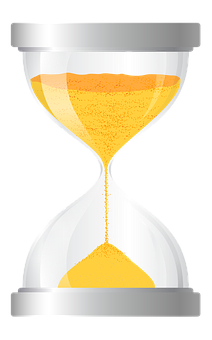
\includegraphics[width=1\textwidth]{Ampulheta}
        \end{figure}}
\end{frame}

\begin{frame}
    \frametitle{Recursos valiosos}
    \begin{itemize}
        \item Algoritmos demandam tempo de execução e recursos:
              \begin{itemize}
                  \item Memória
                  \item Espaço em disco
                  \item Dispositivos externos
                  \item Banda de rede
                  \item \ldots
              \end{itemize}
        \item Um bom programador deve ter o atributo de \textbf{poupar} tempo e recursos.
        \item A principal desempenho avaliado é a \emph{economia} do tempo necessário para o cálculo dos algoritmos.
    \end{itemize}
\end{frame}

\newcommand{\randomGrid}[1]{%
    \begin{tikzpicture}[scale=1]
        \def\gridSize{#1}
        \foreach \x in {1,...,\gridSize} {
                \foreach \y in {1,...,\gridSize} {
                        \pgfmathsetmacro{\randomColor}{rnd}
                        \pgfmathsetmacro{\randomNumber}{int(random(1,1000))}
                        \fill[red!20] (\x-1,\y-1) rectangle (\x,\y);
                        \node at (\x-0.5,\y-0.5) {\randomNumber};
                    }
            }
        \draw[step=1cm, fill=blue] (0,0) grid (\gridSize,\gridSize);
    \end{tikzpicture}%
}

\begin{frame}\frametitle{Quanto tempo preciso para organizar este grid?}
    \begin{center}
        \randomGrid{2}
    \end{center}
\end{frame}

\begin{frame}
    \frametitle{Quanto tempo preciso para organizar este grid?}
    \begin{center}
        \randomGrid{3}
    \end{center}
\end{frame}

\begin{frame}
    \frametitle{Quanto tempo preciso para organizar este grid?}
    \begin{center}
        \randomGrid{4}
    \end{center}
\end{frame}

\begin{frame}
    \frametitle{Quanto tempo preciso para organizar este grid?}
    \begin{center}
        \randomGrid{5}
    \end{center}
\end{frame}

\newcommand{\figuraRegular}[2]{%
    \begin{center}
        \begin{tikzpicture}
            \pgfmathsetmacro{\radius}{#2} % Raio da figura regular
            \pgfmathsetmacro{\angle}{360/#1} % Ângulo entre os lados da figura regular
            \pgfmathsetmacro{\apothem}{\radius*cos(\angle/2)} % Apótema da figura regular

            % Desenhar os vértices da figura regular
            \foreach \i in {1,...,#1} {
                    \pgfmathsetmacro{\x}{\radius*cos(\i*\angle)}
                    \pgfmathsetmacro{\y}{\radius*sin(\i*\angle)}
                    \coordinate (v\i) at (\x,\y);
                }

            % Desenhar a figura regular
            \draw (v1)
            \foreach \i in {2,...,#1} {
                    -- (v\i)
                } -- cycle;

            % Desenhar o apótema
            \draw[dashed] (0,0) -- (v1) node[midway, above] {};
            \draw[dashed] (0,0) -- (v2) node[midway, above] {};

            \node[anchor=west, xshift=1cm, text width=8cm] at (0.5,0) {
                \pgfmathsetmacro{\alfa}{(180 - (360/#1))/2}
                \pgfmathsetmacro{\alfaB}{tan(\alfa)}
                \pgfmathsetmacro{\Atotal}{#1*2*\alfaB/2}
                \pgfmathsetmacro{\diag}{2*sqrt(1+\alfaB*\alfaB)}

                \pgfmathsetmacro{\pAlfa}{round(100*\alfa)/100}
                \pgfmathsetmacro{\pAlfaB}{round(100*\alfaB)/100}
                \pgfmathsetmacro{\pTotal}{round(100*\Atotal)/100}
                \pgfmathsetmacro{\PT}{2*#1}
                \pgfmathsetmacro{\razao}{\PT/\diag}

                \begin{align*}
                    2*\alpha   & = \left(180 - \frac{360}{#1}\right) \rightarrow \alpha   = \pAlfa ^o \\
                    tg(\alpha) & = \frac{h}{L/2}          \rightarrow h                 = \pAlfaB     \\
                    P_T        & = #1L      = \PT                                                     \\
                    D          & = 2\sqrt{1+h^2}= \diag                                               \\
                    \pi        & \approx P_T/D = \razao
                \end{align*}
            };
        \end{tikzpicture}
    \end{center}
}

\newcommand{\slidefiguraRegular}[2]{
    \begin{frame}
        \frametitle{Cálculo do $\pi$ (Alg. 1)}
        \framesubtitle{#2 lados  ($L=2$)}
        \figuraRegular{#2}{#1}
    \end{frame}
}

\foreach \i in {3,...,20} {
        \slidefiguraRegular{2}{\i}
    }

\begin{frame}
    \begin{center}
        \begin{tikzpicture}
            \frametitle{Cálculo do $\pi$ (Alg. 1)}
            \draw[fill=none](0,0) circle (2.0);
            \draw (0,0) -- (2,0) node[midway, yshift=10] {R};
            \node[anchor=west, xshift=1cm, text width=6cm] at (2,0.5) {
                $$\lim_{n\rightarrow\infty}\left(\frac{P_T}{D}\right) = \left(\frac{2 \pi R}{2R}\right)= \pi$$
            };
        \end{tikzpicture}
    \end{center}
\end{frame}


\newcounter{bluePointsCounter}
\newcommand{\circuloEQuadrado}[1]{
    \setcounter{bluePointsCounter}{0}
    \begin{tikzpicture}
        \draw (0,0) rectangle (4,4);
        \draw (2,2) circle [radius=2cm];
        \fill (2,2) circle [radius=0.5pt];
        \foreach \i in {1,...,#1}
            {
                \pgfmathsetmacro{\x}{random()*4}
                \pgfmathsetmacro{\y}{random()*4}

                % Verifica se o ponto está dentro do círculo
                \pgfmathparse{(\x-2)^2 + (\y-2)^2 <= 2^2 ? int(1) : int(0)}
                \ifnum\pgfmathresult=1
                    \fill[blue] (\x,\y) circle [radius=1pt];
                    \stepcounter{bluePointsCounter} % Incrementa o contador
                \else
                    \fill[red] (\x,\y) circle [radius=1pt];
                \fi
            }

        % Exibe o valor do contador
        \def\azul{\thebluePointsCounter}
        \node[anchor=west] at (6,3.5) {Pontos Azuis(A): \thebluePointsCounter};
        \pgfmathsetmacro{\vermelhos}{#1 - \thebluePointsCounter};
        \node[anchor=west] at (6,2.5) {Pontos Vermelhos(V): \vermelhos};
        \node[anchor=west] at (6,1.5) {Totais(T): #1};
        \pgfmathsetmacro{\razao}{4*\azul/#1};
        \node[anchor=west] at (6,0.5) {4*Razão (A/T): \razao};
        \draw[|-|] (0,-0.5) -- node[below] {$L=4$} (4,-0.5);
        \draw[|-|] (2,2) -- node[below] {$R=2$} ++(2,0);
    \end{tikzpicture}
}
\newcommand{\calcpi}[1]{
    \begin{frame}
        \frametitle{Cálculo do $\pi$ (Alg. 2)}
        \circuloEQuadrado{#1}
    \end{frame}
}
\foreach \i in {10,20,...,200} {
        \calcpi{\i}
    }

\begin{frame}[t]
    \frametitle{Cálculo de $\pi$ (Alg. 2)}
    \circuloEQuadrado{50}
    Quando os pontos tendem ao infinito:
    \begin{align*}
        \lim_{N\rightarrow\infty} A/T = \frac{A_c}{A_q} = \frac{\pi R^2}{(2R)^2} = \frac{\pi}{4}
    \end{align*}

\end{frame}

\begin{frame}
    \frametitle{Cálculo da complexidade}
    Tempo de Execução:
    $$T(n) = \sum^n_{i=1} t_in_i$$
    \begin{itemize}
        \item $i$ índice da instrução;
        \item $t_i$ o tempo necessário para a excução da instrução $i$;
        \item $n_i$ o número de vezes que a instrução $i$ é executada.
    \end{itemize}
\end{frame}

\begin{frame}
    \frametitle{Obtenção de $t_i$}\large
    O cálculo de $t_i$ depende:
    \begin{itemize}
        \item Memória disponível do computador;
        \item Desempenho do processador;
        \item Arquitetura e estado dos dispositivos naquele momento de execução.
    \end{itemize}

    \pause Até mesmo o mesmo computador tem tempo de respostas diferentes.

\end{frame}

\begin{frame}
    \frametitle{Experimento para cálculo do tempo}

    \begin{center}

        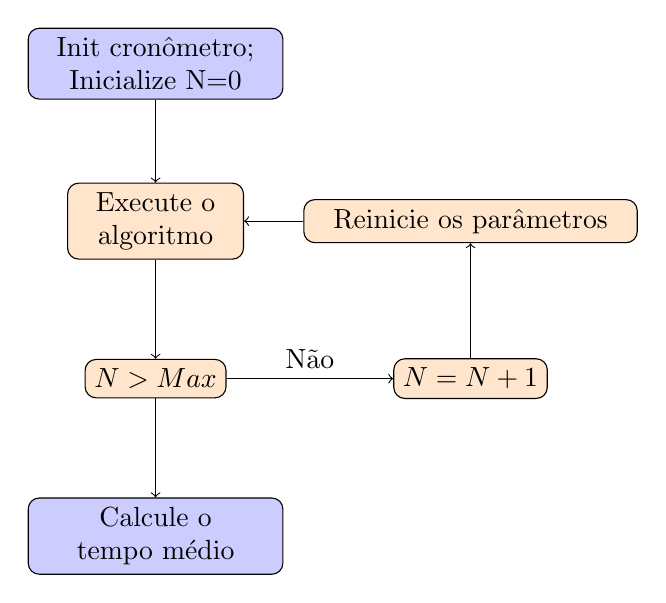
\begin{tikzpicture}[node distance=2cm, every node/.style={rectangle, draw, text centered, rounded corners}]

            % Passo Inicial
            \node<1-> (inicial) [fill=blue!20, rectangle,text width=3cm] {Init cronômetro; Inicialize N=0};

            % Passos Intermediários
            \onslide<2->\node (passo1) [fill=orange!20, below of=inicial, text width=2cm] {Execute o algoritmo};
            \onslide<3->\node (passo2) [fill=orange!20, below of=passo1] {$N>Max$};
            \onslide<6->\node (passo3) [fill=blue!20, below of=passo2,text width=3cm] {Calcule o tempo médio};

            % Conexões
            \onslide<2->\draw [->] (inicial) -- (passo1);
            \onslide<3->\draw [->] (passo1) -- (passo2);
            \onslide<6->\draw [->] (passo2) -- (passo3);

            % Fluxo Alternativo
            \onslide<4->\node (condicao) [fill=orange!20, right of=passo2, node distance=4cm] {$N = N+1$};
            \onslide<5->\node (retorno) [fill=orange!20, above of=condicao, text width=4cm] {Reinicie os parâmetros};

            \onslide<4->\draw [->] (passo2.east) -- node[above, draw=none] {Não} (condicao.west);
            \onslide<5->\draw [->] (condicao.north) -- (retorno.south);
            \onslide<5->\draw [->] (retorno.west) -- (passo1.east);


        \end{tikzpicture}
    \end{center}

\end{frame}

\begin{frame}[fragile, t]
    \frametitle{Contagem de Frequência - Algoritmo 1}

    \begin{lstlisting}[language=C++, basicstyle=\small]
        int main() {
            int x = 0;
            x = x + 1;
            return 0;
        }
  \end{lstlisting}

\end{frame}

\begin{frame}[fragile, t]
    \frametitle{Contagem de Frequência - Algoritmo 2}

    \begin{lstlisting}[language=C++, basicstyle=\small]
        int main() {
            int x = 0, n=10;
            for (int i = 0; i < n; i++) {
                x = x + 1;
            }
            return 0;
        }
  \end{lstlisting}

\end{frame}

\begin{frame}
    \frametitle{Contagem de frequência}
    Exemplo: Conte as operações (contagem de frequência) realizadas na operação de uma soma geométrica definida por:
    $$S = \sum_{i=0}^n x^i$$
    Analise as instruções do algoritmo que o descreve logo a seguir:
\end{frame}

\begin{frame}\normalsize
    \frametitle{Contagem de frequência - Algoritmo 4}
    \duascolunas{\codecppNoTitle[0.9]{algSoma.c}}
    {
        \begin{enumerate}
            \item[L2)] $1$
            \item[L3)] $n+2$
            \item[L4)] $n+1$
            \item[L6)] $\sum_{i=0}^n i$
            \item[L7)] $n+1$
            \item[L9)] $1$
        \end{enumerate}}
    \pause Somando todos os tempos, temos o tempo total:  \begin{center}
        $T(n) = \frac{n^2}{2} + \frac{7n}{2} + 6$
    \end{center}
\end{frame}

\begin{frame}
    \frametitle{Fórmula de \textit{Horner}}

    Pode-se modificar o algoritmo para melhorar o tempo de execução utilizando o algoritmo de \emph{Horner}.
    \begin{align*}
        S = \sum_{i=0}^n x^i & = 1 + x + x^2 +\ldots + x^n                 \\
                             & = 1+x(1 + x + x^2 +\ldots + x^{n-1})        \\
                             & = 1+x(1 + x(1 + x + x^2 +\ldots + x^{n-2})) \\
                             & = 1+x(1+x(1+ x(1+\ldots(1+x(1+x)))\ldots))
    \end{align*}
\end{frame}

\begin{frame}
    \frametitle{Contagem de frequência - Algoritmo 5}
    \duascolunas{\codecppNoTitle[0.9]{algSoma2.c}}{
        \begin{enumerate}
            \pause\item[L2)] 1
                \pause\item [L3)] n+2
                  \pause\item [L4)] n+1
                  \pause\item [L6)] 1
        \end{enumerate}}
    \vfill
    \pause\centering Portanto: $T(n) = 1+(n+2)+(n+1)+1 = 2n+5$.
\end{frame}

\begin{frame}
    \frametitle{Fórmula fechada}
    Uma terceira solução é encontrar a fórmula fechada:
    \begin{align*}
        \onslide<1-> {S = \sum_{i=0}^n i & = 1 + x + x^2 +\ldots + x^n}    \\
        \onslide<2->{xS                  & = x(1 + x + x^2 +\ldots + x^n)} \\
        \onslide<3->{xS                  & = x + x^2 +\ldots + x^{n+1}}    \\
        \onslide<4->{xS +1               & = 1+x + x^2 +\ldots + x^{n+1}}  \\
        \onslide<5->{xS +1               & = S + x^{n+1}}                  \\
        \onslide<6->{xS -S               & = x^{n+1}-1}                    \\
        \onslide<7->{(x-1)S              & = x^{n+1}-1}                    \\
        \onslide<8->{S                   & = \frac{x^{n+1}-1}{x-1}}
    \end{align*}
\end{frame}

\begin{frame}
    \frametitle{Contagem de frequência - Algoritmo 6}
    Qual a complexidade desse algoritmo com a fórmula fechada?\vfill

    \pause\codecppNoTitle[0.9]{algSoma3.c}
    \begin{flushleft}
        \pause Considerando que \emph{pow} tem complexidade logaritmica: $$T(n) = log_2 (n+1)$$
    \end{flushleft}
\end{frame}

\begin{frame}
    \frametitle{Equações }
    \begin{center}

        \begin{tikzpicture}[x=8mm, y=0.7mm]
            % Eixos
            \draw[->,line width=0.25pt] (-1,0) -- (10,0) node[right] {n};
            \draw[->,line width=0.25pt] (1,-10) -- (1,80) node[above] {f(n)};
            \draw[xshift=-14pt] (1,0.1) -- (1,-0.1) node[below] {(1,1)};

            \draw<2->[domain=1:8, smooth=bezier, variable=\x, black,line width=0.5pt]
            plot ({\x},{(\x*\x)/2 + (7*\x)/2 + 6}) node[right] {$\frac{n^2}{2} + \frac{7n}{2} + 6$};
            \draw<3->[domain=1:8, smooth=bezier, variable=\x, black,line width=0.5pt]
            plot ({\x},{2*\x + 5}) node[right, yshift=15] {$2n + 5$};
            \draw<4->[domain=1:8, smooth=bezier, variable=\x, black,line width=0.5pt]
            plot ({\x},{log10(\x+1)}) node[right, yshift=15] {$\log(n+1)$};
        \end{tikzpicture}

    \end{center}
\end{frame}

\newcolumntype{P}[1]{>{\centering\arraybackslash}p{#1}}
\renewcommand{\arraystretch}{1.5}
\begin{frame}
    \frametitle{Comportamento assintótico}
    Comparação numérica da complexidade: Considere que cada operação ($n=1$) dura/custa\footnote{Dura/custa: Termo de comparação dos algoritmos} de $0.0001s = 100\mu s$.\vfill
    \begin{table}[]
        \begin{tabular}{P{2.5cm}P{2.5cm}P{2.5cm}P{2.5cm}}
            $T(n)$      & $20$                 & $40$                       & $60$                                                                                                                         \\ \hline
            $n$         & \only<2->{$200\mu s$ & $400\mu s$                 & $600\mu s$}                                                                                                                  \\ \hdashline
            $n\ log(n)$ & \only<3->{$900\mu s$ & $2.1ms$                    & $3.5ms$}                                                                                                                     \\ \hdashline
            $n^2$       & \only<4->{$4ms$      & $16ms$                     & $36ms$}                                                                                                                      \\ \hdashline
            $n^3$       & \only<5->{$80ms$     & $640ms$                    & $2.16s$}                                                                                                                     \\ \hdashline
            $2^n$       & \only<6->{$10s$      & $27 dias$}   \only<7->{    & $3660$ séculos}                                                                                                              \\ \hdashline
            $3^n$       & \only<8->{$580min$}  & \only<9->{$38550$ séculos} & \only<10->{$1.3*10^{14}$ séculos\footnote{O tempo do universo medido em séculos é de aproximadamente $13.8*10^{7}$ séculos}}
        \end{tabular}
    \end{table}
\end{frame}


\definecolor{olivegreen}{RGB}{85, 107, 47}
\begin{frame}[t]
    \frametitle{Complexidade Assintótica}
    \large O que significa complexidade assintótica?
    \begin{center}
        \begin{tikzpicture}[x=50]
            % Eixo x
            \draw<1->[->, line width=1] (0,0) -- (5,0) node[right] {$n$};
            \draw<1->[->, line width=1] (0,0) -- (0,5) node[above] {$f(n)$};
            \draw<2->[smooth, blue, line width=0.5] plot coordinates {(0,0) (1,1) (2,3) (3,2.5) (4,4) (5,5)};
            \draw<3-6>[smooth, red, line width=0.5] plot coordinates {(0,0) (1,2) (2,2) (3,2) (4,3) (5,3)};
            \draw<4-6>[smooth, olivegreen, line width=0.5] plot coordinates {(0,0) (1,1) (2,3) (3,2) (4,2) (5,2)};
            \draw<7>[smooth, red!20, line width=0.5] plot coordinates {(0,0) (1,2) (2,2) (3,2) (4,3) (5,3)};
            \draw<7>[smooth, olivegreen!20, line width=0.5] plot coordinates {(0,0) (1,1) (2,3) (3,2) (4,2) (5,2)};
            \draw<5>[-, line width=1, dashed] (3,5) -- (3,0) node[below] {$n=3$};
            \draw<6>[-, line width=1, dashed] (2,5) -- (2,0) node[below] {$n=2$};
            \draw<7->[smooth, blue, line width=1.5] plot coordinates {(0,0) (1,1) (2,3) (3,2.5) (4,4) (5,5)};
        \end{tikzpicture}
    \end{center}
\end{frame}

\begin{frame}[t]
    \frametitle{Assíntota}
    \framesubtitle{O que é uma assíntota?}
    São retas horizontais ou verticais que determinam a aproximação das curvas.
    \begin{beamerboxesrounded}{Exemplo}
        \begin{enumerate}[label=\alph*)]
            \setlength\itemsep{1em}
            \item $f(x) = \frac{3x}{x-1}$
            \item $f(x) = \frac{1}{(x-2)^2}$
            \item $f(x) = \frac{(x+2)(x-1)}{x(x+1)(x-2)}$
            \item $f(x) = \frac{x}{\sqrt{x^2+2}}$
            \item $f(x) = 1+e^{-x}$
            \item $f(x) = \log\left(2+3^x\right)$
        \end{enumerate}
    \end{beamerboxesrounded}

\end{frame}

\begin{frame}[t]
    \frametitle{Complexidade Assintótica}
    % \framesubtitle{Notação $O(n)$}
    \begin{beamerboxesrounded}{Definição}
        Uma função $g(n)$ \textbf{domina assintoticamente} outra função f(n) se existem duas constantes positivas $c$ e $m$ tais que, para $n\geq m$, tem-se $$\left|f(n)\right| \leq c\times \left|g(n)\right|$$
    \end{beamerboxesrounded}

    \pause\begin{center}
        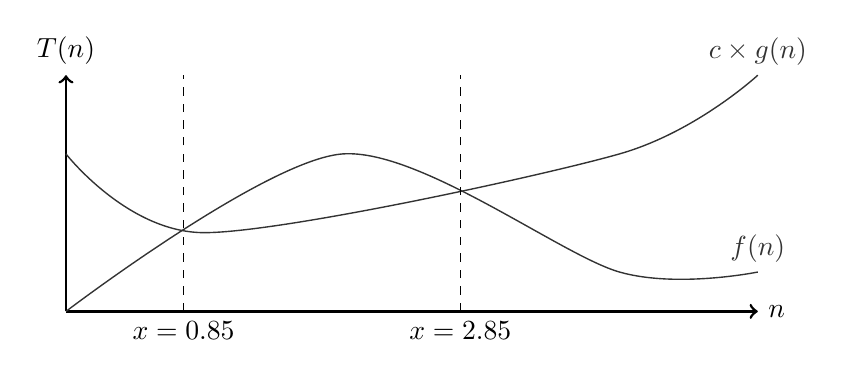
\begin{tikzpicture}[x=50]
            % Eixo x
            \draw[->, line width=1] (0,0) -- (5,0) node[right] {$n$};
            \draw[->, line width=1] (0,0) -- (0,3) node[above] {$T(n)$};
            \draw[smooth, black!80, line width=0.5] plot coordinates {(0,0) (2,2) (4,0.5) (5, 0.5)} node[above] {$f(n)$};
            \draw[smooth, black!80, line width=0.5] plot coordinates {(0,2) (1,1) (4,2) (5, 3)} node[above] {$c\times g(n)$};
            \draw[thin, dashed] (2.85, 0) node[below] {$x=2.85$} -- (2.85, 3);
            \draw[thin, dashed] (0.85, 0) node[below] {$x=0.85$} -- (0.85, 3);
        \end{tikzpicture}
    \end{center}
\end{frame}

\begin{frame}[t]
    \frametitle{Assíntota}
    \framesubtitle{Domínio assintótico}
    \begin{beamerboxesrounded}{Determine quais funções são dominantes:}
        \begin{enumerate}[label=\alph*)]
            \setlength\itemsep{1em}
            \item $f(n)=n$ ou $g(n)=-n^2$
            \item $f(n)=50n$ ou $g(n)=2n^2$
            \item $f(n)=(n+1)^2$ ou $g(n)=n^2$
            \item $f(n)=n^2 + 2n + 1$ ou $g(n)=0.1n^3$
            \item $f(n)=0.2n^2$ ou $g(n)=1000n$
        \end{enumerate}
    \end{beamerboxesrounded}
\end{frame}

\begin{frame}[t]
    \frametitle{Complexidade Assintótica}
    \begin{itemize}
        \item Na análise de algoritmos, geralmente usa-se a complexidade assintótica, analisando o algoritmo para n tendendo a infinito;
        \item Nesse caso, despreza-se constantes e termos de menor crescimento;
        \item Usa-se notações especiais para a complexidade assintótica.
    \end{itemize}
    \pause Tipos de Notação:
    \pause\begin{center}

        \begin{tabular}{c|c}
            \textbf{Notação}   & \textbf{Descrição simplificada} \\
            \hline
            \pause $O(n)$      & Limitador Estrito Superior      \\
            \pause $\Omega(n)$ & Limitador Estrito Inferior      \\
            \pause $\Theta(n)$ & Limitador Central               \\
            \pause $o(n)$      & Limitador Não Estrito Superior  \\
            \pause $\omega(n)$ & Limitador Não Estrito Inferior  \\
            \hline
        \end{tabular}
    \end{center}
\end{frame}

\begin{frame}[t]
    \frametitle{Notação $O$}
    Uma função $f(n)$ é dita como sendo $O(g(n))$ se existe uma constante positivas $c$ para o qual:

    $$0<f(n) \leq c\times g(n)$$

    para todo $n>n_0$.

    \begin{center}
        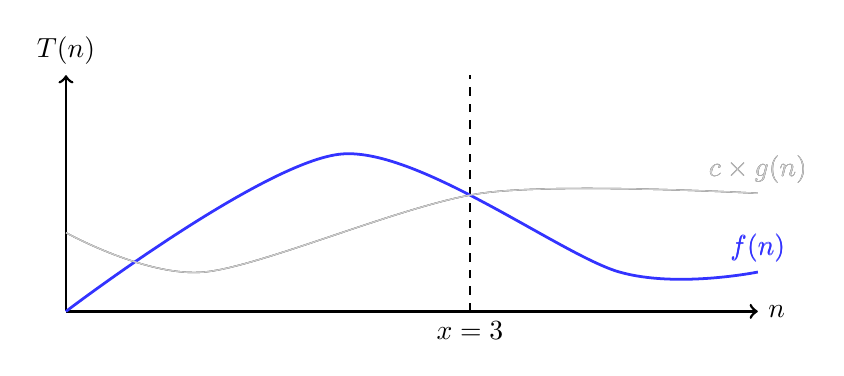
\begin{tikzpicture}[x=50]
            \draw<1->[->, line width=1] (0,0) -- (5,0) node[right] {$n$};
            \draw<1->[->, line width=1] (0,0) -- (0,3) node[above] {$T(n)$};

            % Curva preta
            \draw<3-4>[smooth, black!80, line width=0.5] plot coordinates
                {(0,1) (1,0.5) (3,1.5) (5, 1.5)} node[above] {$c\times g(n)$};
            % Curva azul forte
            \draw<2->[smooth, blue!80, line width=0.5] plot coordinates
                {(0,0) (2,2) (4,0.5) (5, 0.5)} node[above] {$f(n)$};
            % Assíntota
            \draw<4->[thin, dashed] (2.92, 0) node[below]
            {$x=3$} -- (2.92, 3);
            \draw<5->[smooth, blue!80, line width=1.0] plot coordinates
                {(0,0) (2,2) (4,0.5) (5, 0.5)} node[above] {$f(n)$};
            % Curva preta
            \draw<5->[smooth, black!20, line width=0.5] plot coordinates
                {(0,1) (1,0.5) (3,1.5) (5, 1.5)} node[above] {$c\times g(n)$};
            % \draw[smooth, blue!80, line width=1] plot coordinates  
            %   {(0,1) (1,0.5) (3,1.5) (5, 1.5)} node[above] {$f(n)$};
        \end{tikzpicture}
    \end{center}
\end{frame}

\begin{frame}[t]
    \frametitle{Notação $\Omega$}
    Uma função $f(n)$ é dita como sendo $O(g(n))$ se existe uma constante positivas $c$ para o qual:
  
    $$0< c\times g(n)\leq f(n)$$
  
    para todo $n>n_0$.
  
    \begin{center}
      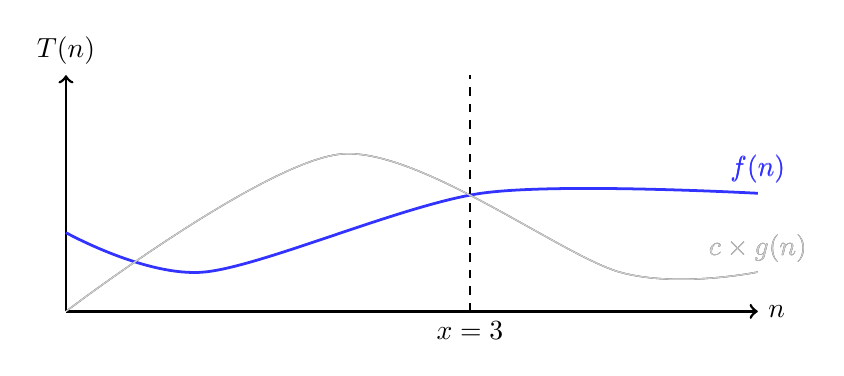
\begin{tikzpicture}[x=50]
        \draw<1->[->, line width=1] (0,0) -- (5,0) node[right] {$n$};
        \draw<1->[->, line width=1] (0,0) -- (0,3) node[above] {$T(n)$};
  
        % Curva preta
        \draw<3-4>[smooth, black!80, line width=0.5] plot coordinates
          {(0,0) (2,2) (4,0.5) (5, 0.5)} node[above] {$c\times g(n)$};
        % Curva azul forte
        \draw<2->[smooth, blue!80, line width=0.5] plot coordinates
          {(0,1) (1,0.5) (3,1.5) (5, 1.5)} node[above] {$f(n)$};
        % Assíntota
        \draw<4->[thin, dashed] (2.92, 0) node[below]
        {$x=3$} -- (2.92, 3);
        \draw<5->[smooth, blue!80, line width=1.0] plot coordinates
          {(0,1) (1,0.5) (3,1.5) (5, 1.5)}   node[above] {$f(n)$};
        % Curva preta
        \draw<5->[smooth, black!20, line width=0.5] plot coordinates
          {(0,0) (2,2) (4,0.5) (5, 0.5)}node[above] {$c\times g(n)$};
        % \draw[smooth, blue!80, line width=1] plot coordinates  
        %   {(0,1) (1,0.5) (3,1.5) (5, 1.5)} node[above] {$f(n)$};
      \end{tikzpicture}
    \end{center}
  \end{frame}
  
\begin{frame}[t]
    \frametitle{Notação $\Theta$}
    Uma função $f(n)$ é dita como sendo $\Theta(g(n))$ se existem constantes positivas $c_1$, $c_2$ e $n_0$ para os quais:

    $$0<c_1g(n) \leq f(n)\leq c_2g(n)$$

    para todo $n>n_0$.

    \begin{center}
        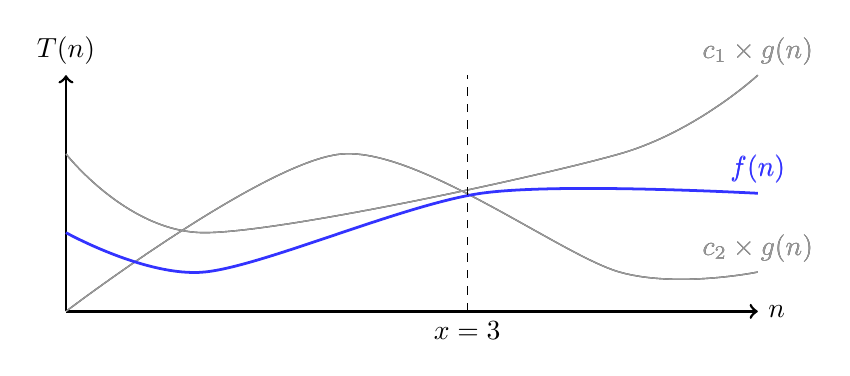
\begin{tikzpicture}[x=50]
            % Eixo x
            \draw<1->[->, line width=1] (0,0) -- (5,0) node[right] {$n$};
            \draw<1->[->, line width=1] (0,0) -- (0,3) node[above] {$T(n)$};
            \draw<2-4>[smooth, black!80, line width=0.5] plot coordinates {(0,2) (1,1) (4,2) (5, 3)} node[above] {$c_1\times g(n)$};
            \draw<3-4>[smooth, black!80, line width=0.5] plot coordinates {(0,0) (2,2) (4,0.5) (5, 0.5)} node[above] {$c_2\times g(n)$};
            \draw<4->[smooth, blue!80, line width=0.5] plot coordinates  {(0,1) (1,0.5) (3,1.5) (5, 1.5)} node[above] {$f(n)$};
            \draw<5->[smooth, black!40, line width=0.5] plot coordinates {(0,2) (1,1) (4,2) (5, 3)} node[above] {$c_1\times g(n)$};
            \draw<5->[smooth, black!40, line width=0.5] plot coordinates {(0,0) (2,2) (4,0.5) (5, 0.5)} node[above] {$c_2\times g(n)$};
            \draw<6->[smooth, blue!80, line width=1] plot coordinates  {(0,1) (1,0.5) (3,1.5) (5, 1.5)} node[above] {$f(n)$};
            \draw<6->[thin, dashed] (2.9, 0) node[below] {$x=3$} -- (2.9, 3);
        \end{tikzpicture}
    \end{center}
\end{frame}

\end{document}

